\subsubsection*{Il piano inclinato}

Dal rotolamento lungo il piano inclinato è possibile trarre ancora altre considerazioni.
Ad esempio, abbiamo osservato che, nel fenomeno interviene la forza di gravità. Ma non in modo diretto, perché le accelerazioni sono molto deboli, a causa dell'inclinazione del piano, pressoché impercettibile e perché la direzione della gravità, in assenza dello stesso piano, darebbe del tutto diversa.\newline

Il motivo per cui una pila accelera lungo la superfice del piano, è in realtà l'effetto di due cause diverse:\newline

\begin{itemize}
\item L'accelerazione di gravità diretta verso il basso;
\item La {\bf reazione vincolare} del piano inclinato, che è diretta in modo ortogonale alla superficie.
\end{itemize}

La funzione di un piano rigido, in effetti, è quello di impedire agli oggetti di attraversarlo. Questo significa che il piano è una struttura capace di esercitare una forza in direzione ortogonale alla superficie stessa. La funzione della gravità, invece, è quella di provocare la caduta dei corpi, cioè un moto diretto verso il entro della terra.

L'accellerazione della pila, al contrario, possiede una direzione diversa dalle casue che la hanno generata, come accade quando si esegue una somma vettoriale. Al contrario, siccome un vettore di un piano può essere scomposto in un modo unico lungo due direttrici indipendenti del piano stesso, è possibile ricavare la gravità e la reazione vincolare del piano scomponendo il vettore che rappresenta l'accelerazione della pila, come nella figura qui sotto:

\begin{figure}[H]
 \centering
 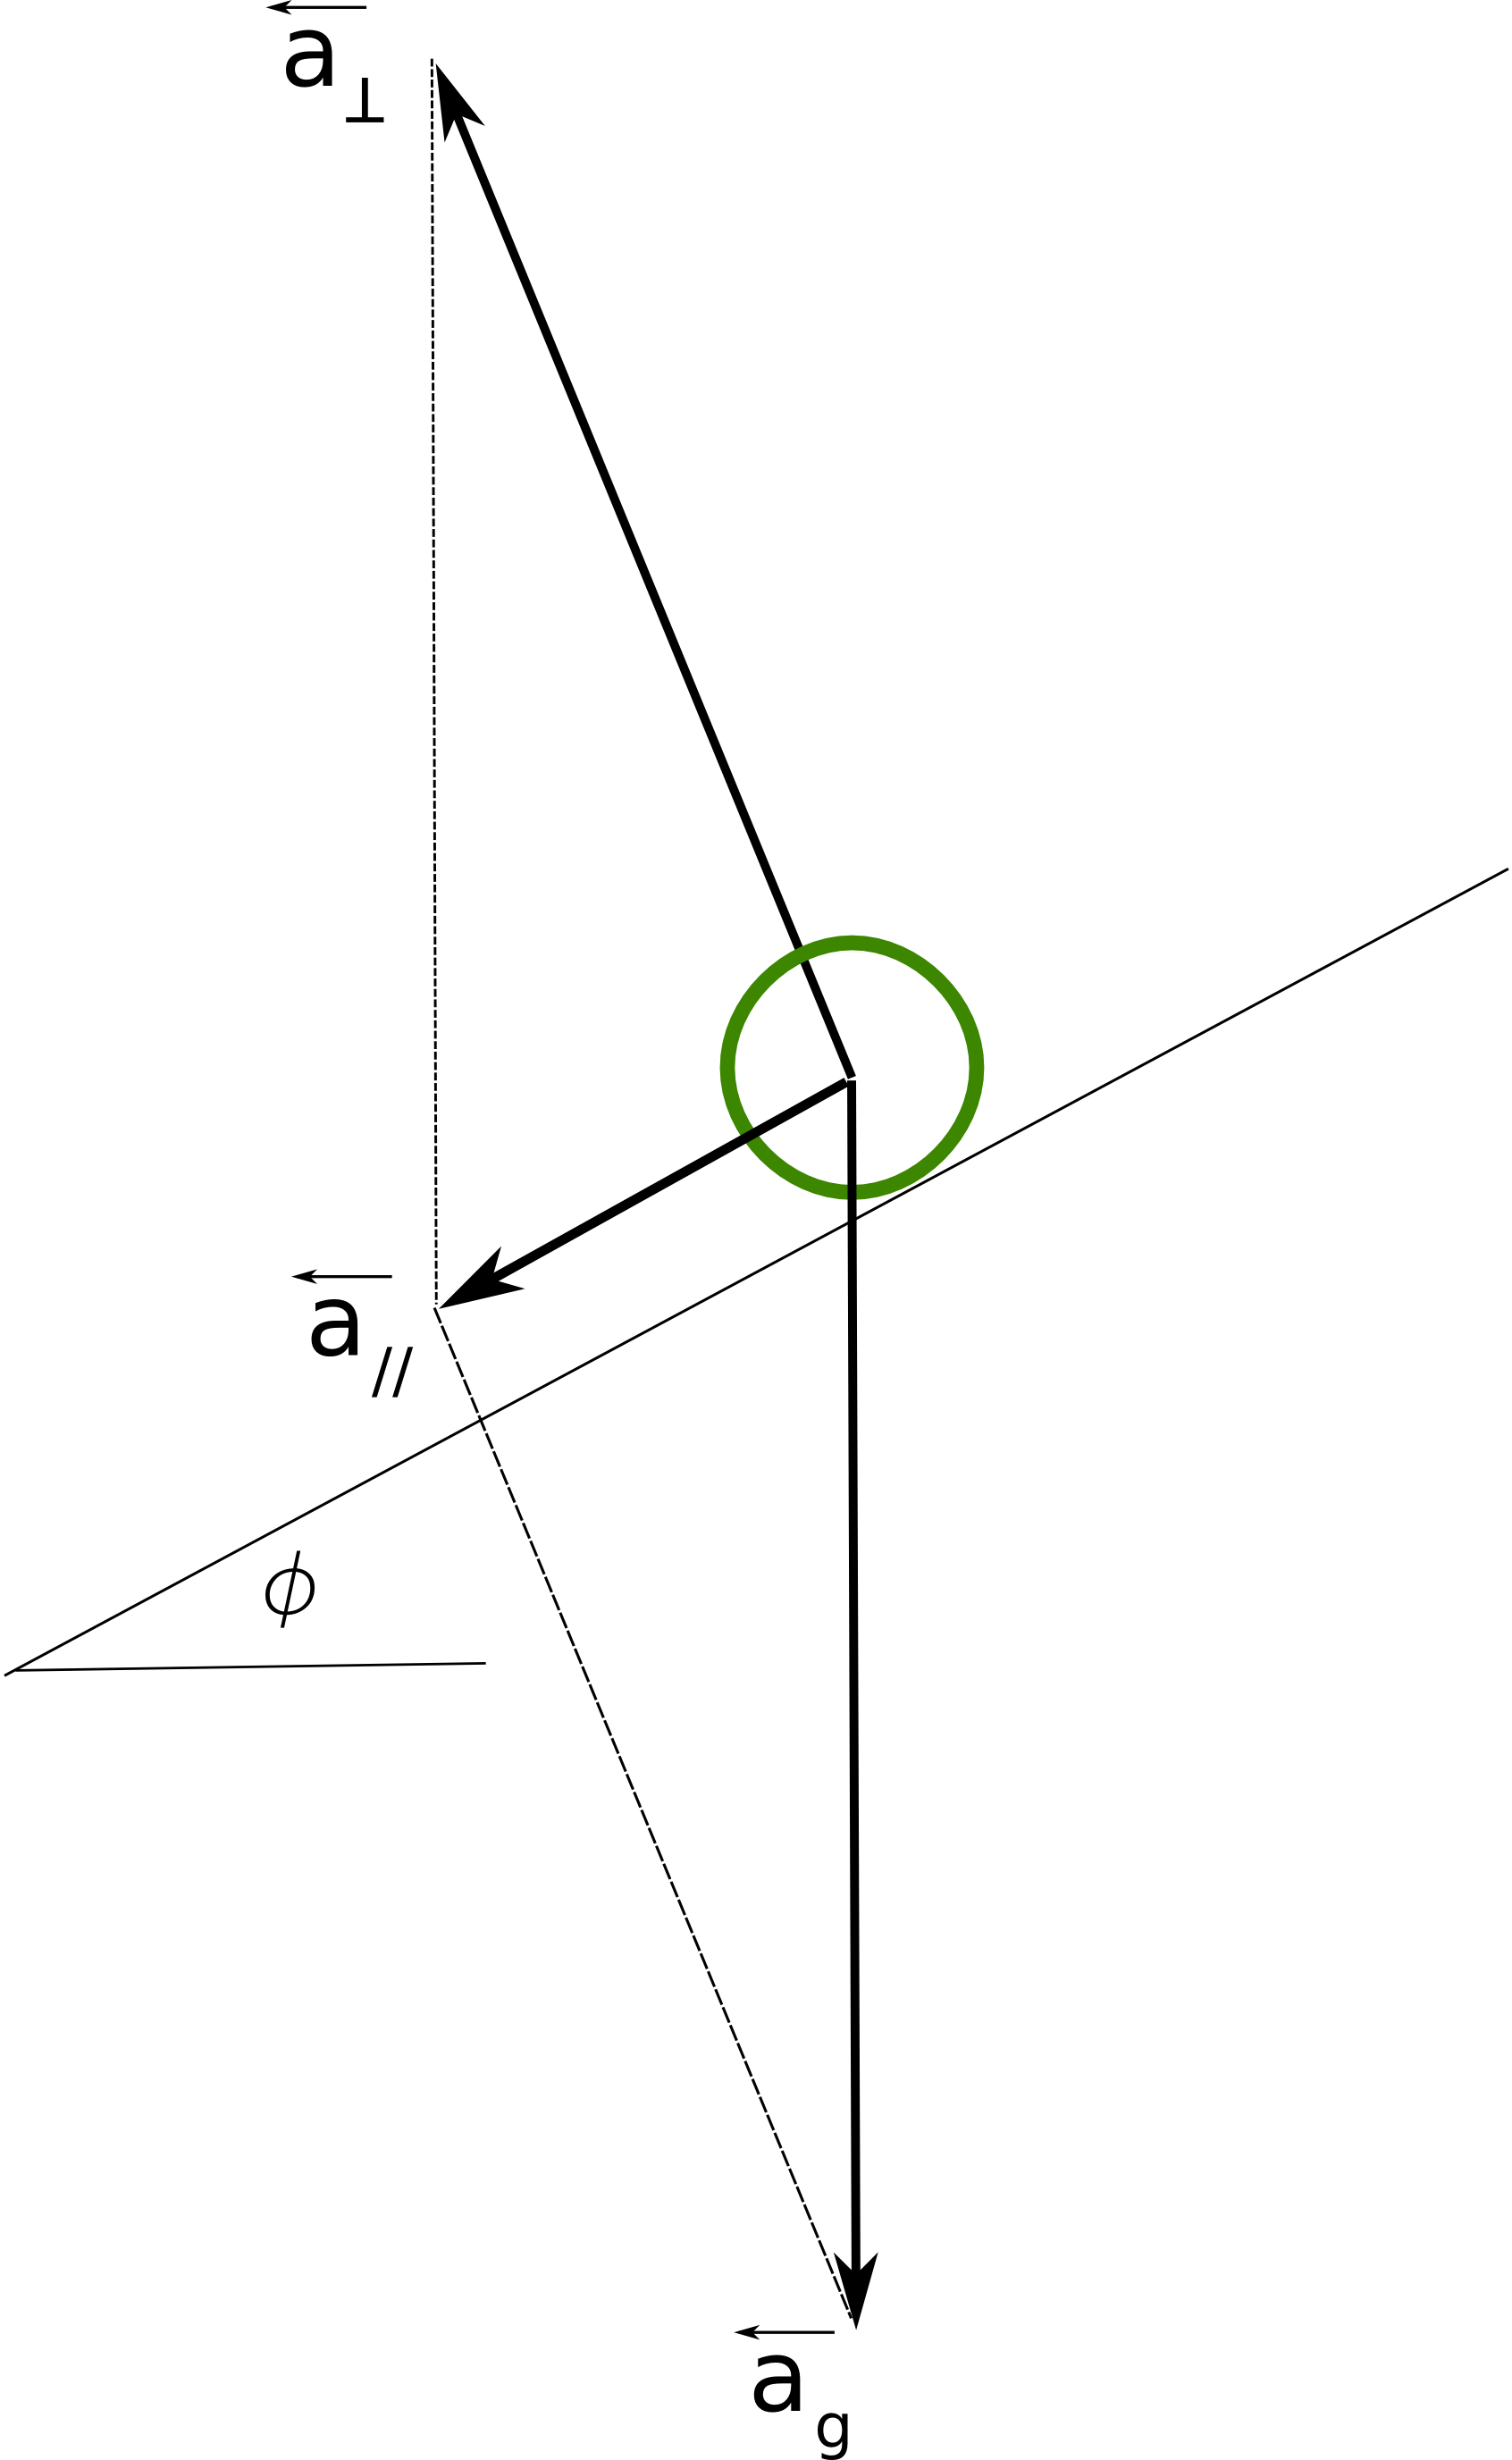
\includegraphics[width=.3\textwidth]{../immagini/gravitaEvincolo.png}
 \label{fig:gravita e reazione vincolare}
\end{figure}

come si può vedere, la relazione tra le accelerazioni in gioco dipende dall'inclinazione $\phi$ del piano, e risulta:

\begin{center}
\begin{math}
\left\{
\begin{array}{r}
a_{//} = a_g sen \phi \\
a_{\perp} = a_g cos \phi
\end{array}
\right.
\end{math}
\end{center}

